\documentclass[11pt]{article}

%\usepackage[utf8]{inputenc}
\usepackage{amsmath}
\usepackage{fancyhdr}
\usepackage{float}
\usepackage{graphicx}
\usepackage[font=small,labelfont=bf]{caption}
\usepackage{booktabs}
\usepackage{microtype}
\usepackage[margin=1in, headheight=2in, top=2in]{geometry}

\chead{%
  {\vbox{%
      \vspace{2mm}
      \large
      Machine Learning \& Data Mining \hfill
      Caltech CS/CNS/EE 155 \hfill \\[1pt]
      Miniproject 3\hfill
      Released March $3^{\text{th}}$, 2017 \\
    }
  }
}

\begin{document}
\pagestyle{fancy}

\section*{Introduction}
\begin{itemize}
\item \underline{\textbf{Group Members}}

Andrew Wang, Steven Brotz, and David LeBaron
\item \underline{\textbf{Team Name}}

Double Boost
\end{itemize}

\section*{Basic Visualizations}
\subsection*{All Ratings}
\begin{figure}[H]
	\centering
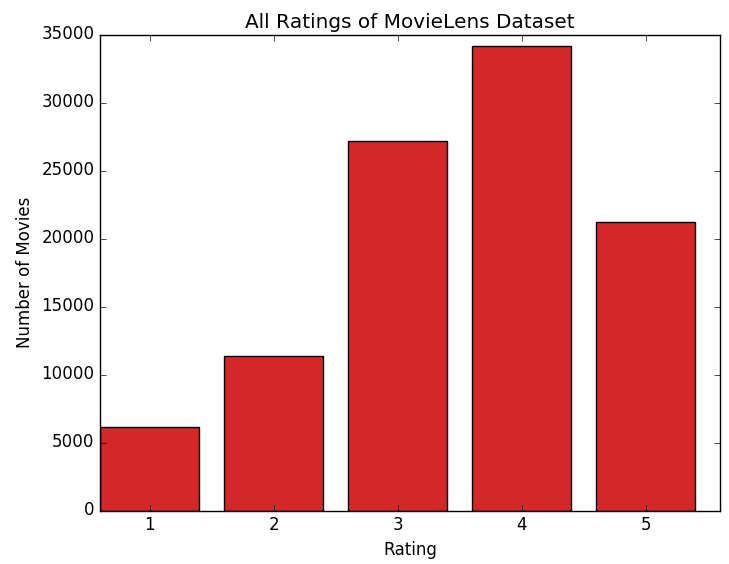
\includegraphics[width=12cm]{AllRatingsBarGraph}
\caption{All ratings of all movies in MovieLens dataset}
\end{figure}
\noindent In order to visualize all ratings, we used a simple bar graph, showing how many movies were rated each rating (1-5). It is immediately clear that 4 is the most common rating given, with almost 10,000 more ratings than the next most common rating. 3 and 5 are the next most common ratings respectively. These results are what we expect to see, as we expect people to rate only movies that they have seen, and typically, people seek movies that they think they will enjoy. Thus, it is no surprise that ratings are generally positive. 

\subsection*{Ten Most Popular Movies}
\begin{figure}[H]
	\centering
	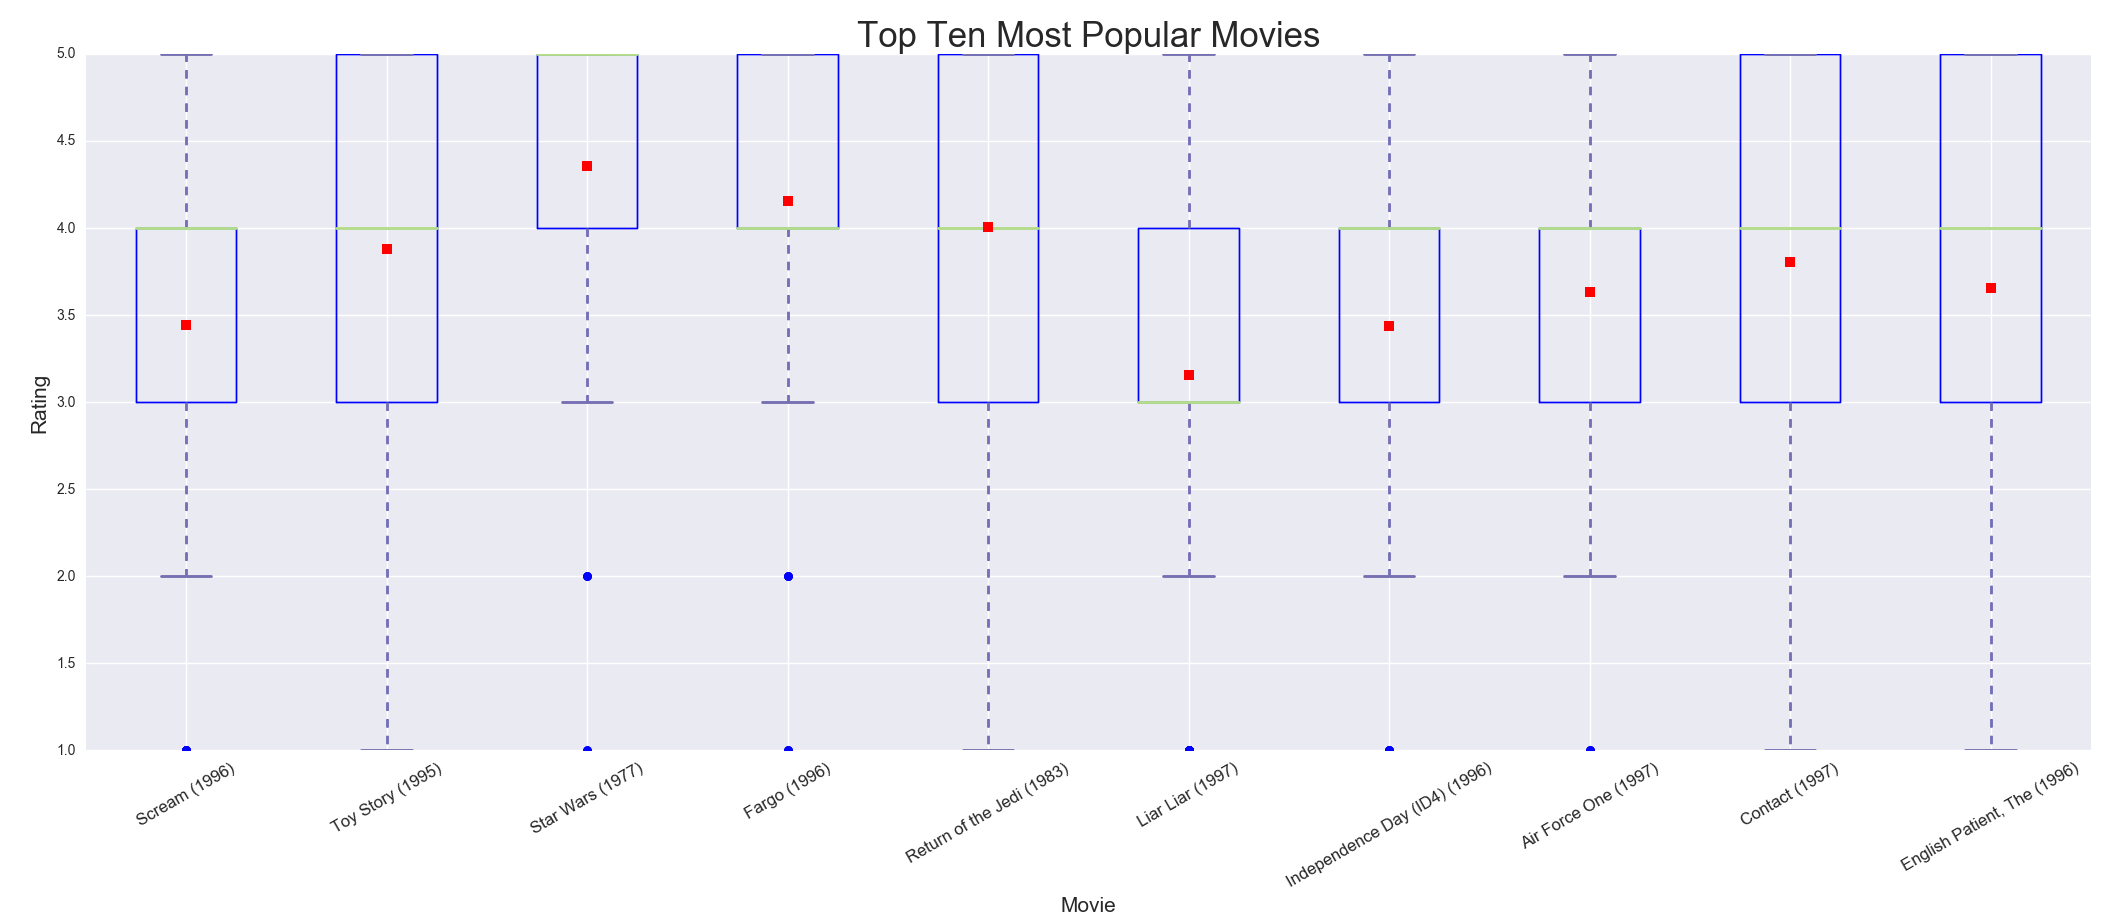
\includegraphics[width=\textwidth]{TopTenPopularBox}
	\caption{Ten most rated movies}
\end{figure}

\begin{figure}[H]
	\centering
	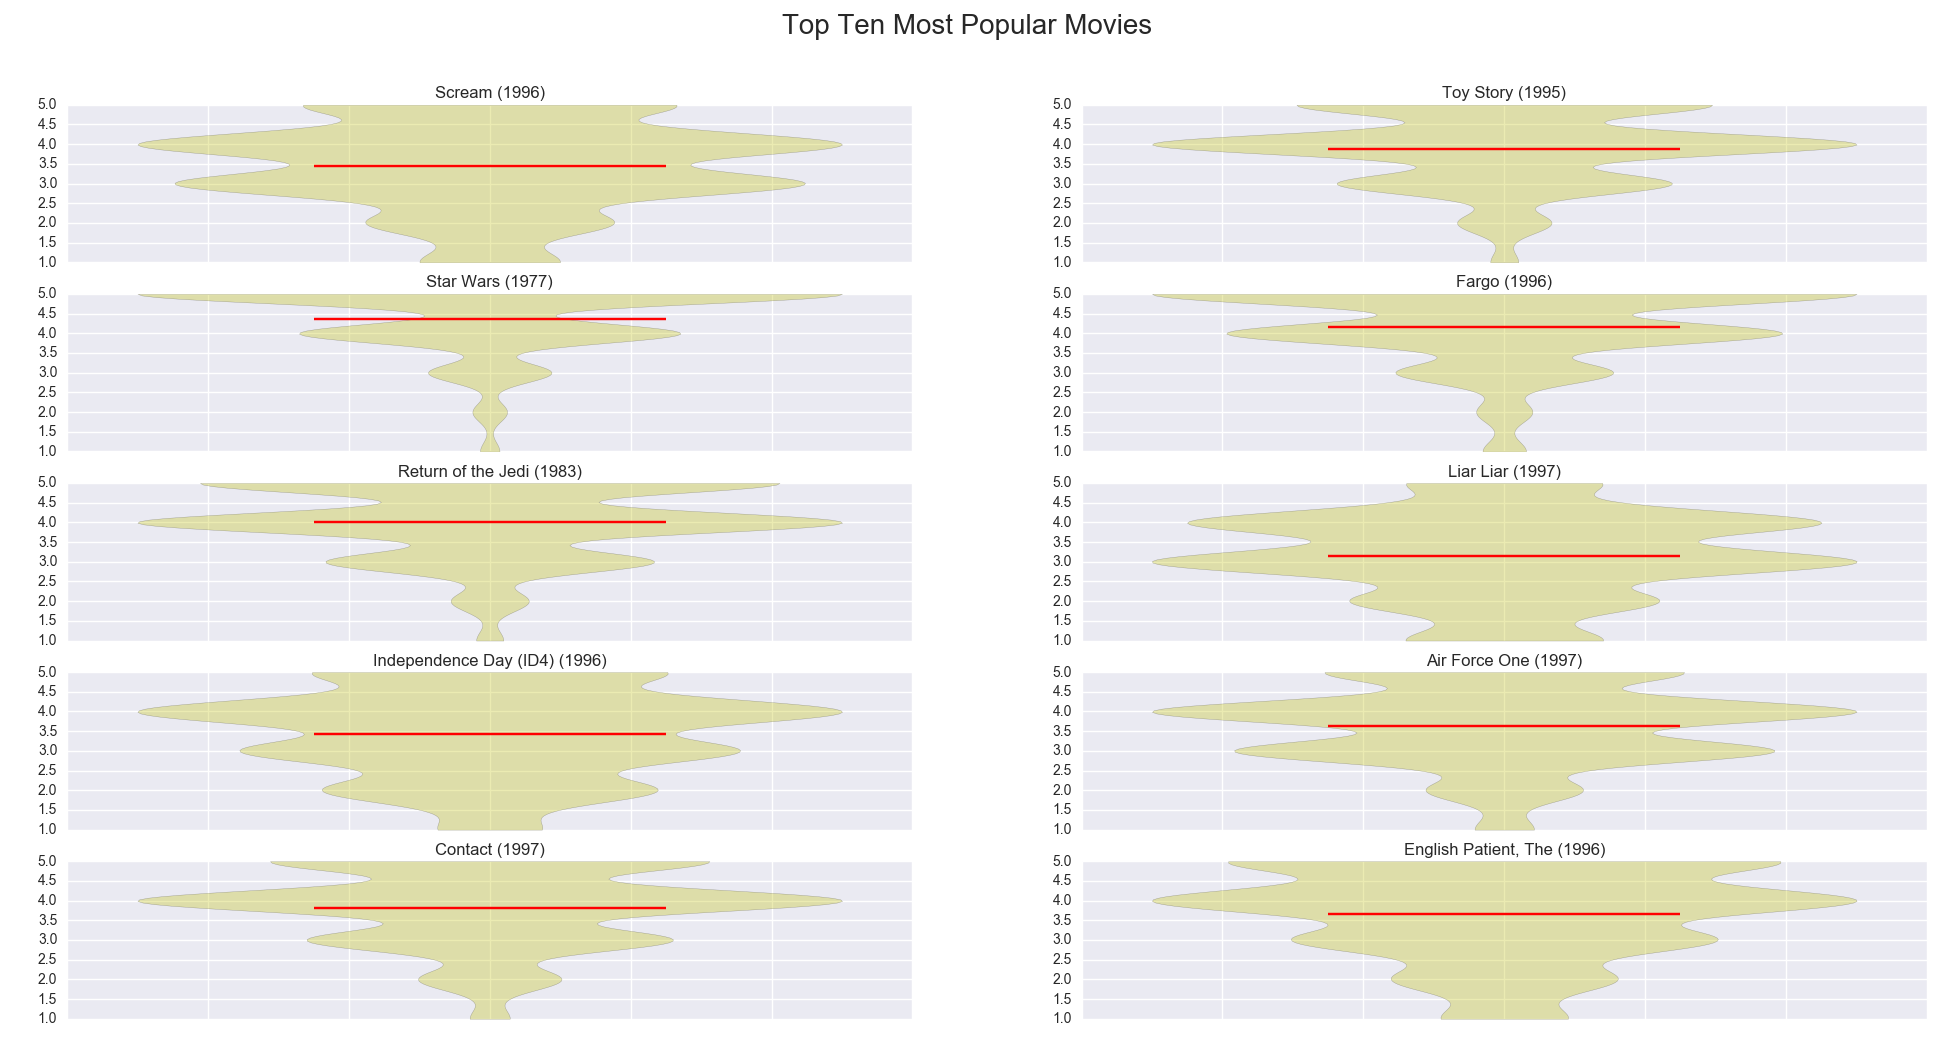
\includegraphics[width=\textwidth]{TopTenPopularSwarm}
	\caption{Ten most rated movies}
\end{figure}

\noindent For the top ten most popular movies (most rated), we utilized box plots and swarm plots. These plots give us a quick way to visualize the overall distribution of ratings for the movies. For the box plot (fig. 2), the green line represents the median while the red dot represents the mean for ratings of each movie. For the swarm plot (fig. 3),the red line represents the mean. In general, we see that there is a good amount of variation in the ratings of these top ten most popular movies, more than the ratings of the top ten best movies (fig. 4,5 below). It is also important to note that the mean and median rating for all these movies are at least 3 which is on the better end of ratings. This makes sense given that popular movies are the most rated and the more people that watch a movie, the more ratings it will get. People tend to watch ``good" movies and ``good" movies generally have good ratings, explaining the overall positive ratings. The unpopular movies are the movies that people tend to not like and thus not watch and thus not rate/rate poorly. 


\subsection*{Ten Best Movies}
\begin{figure}[H]
	\centering
	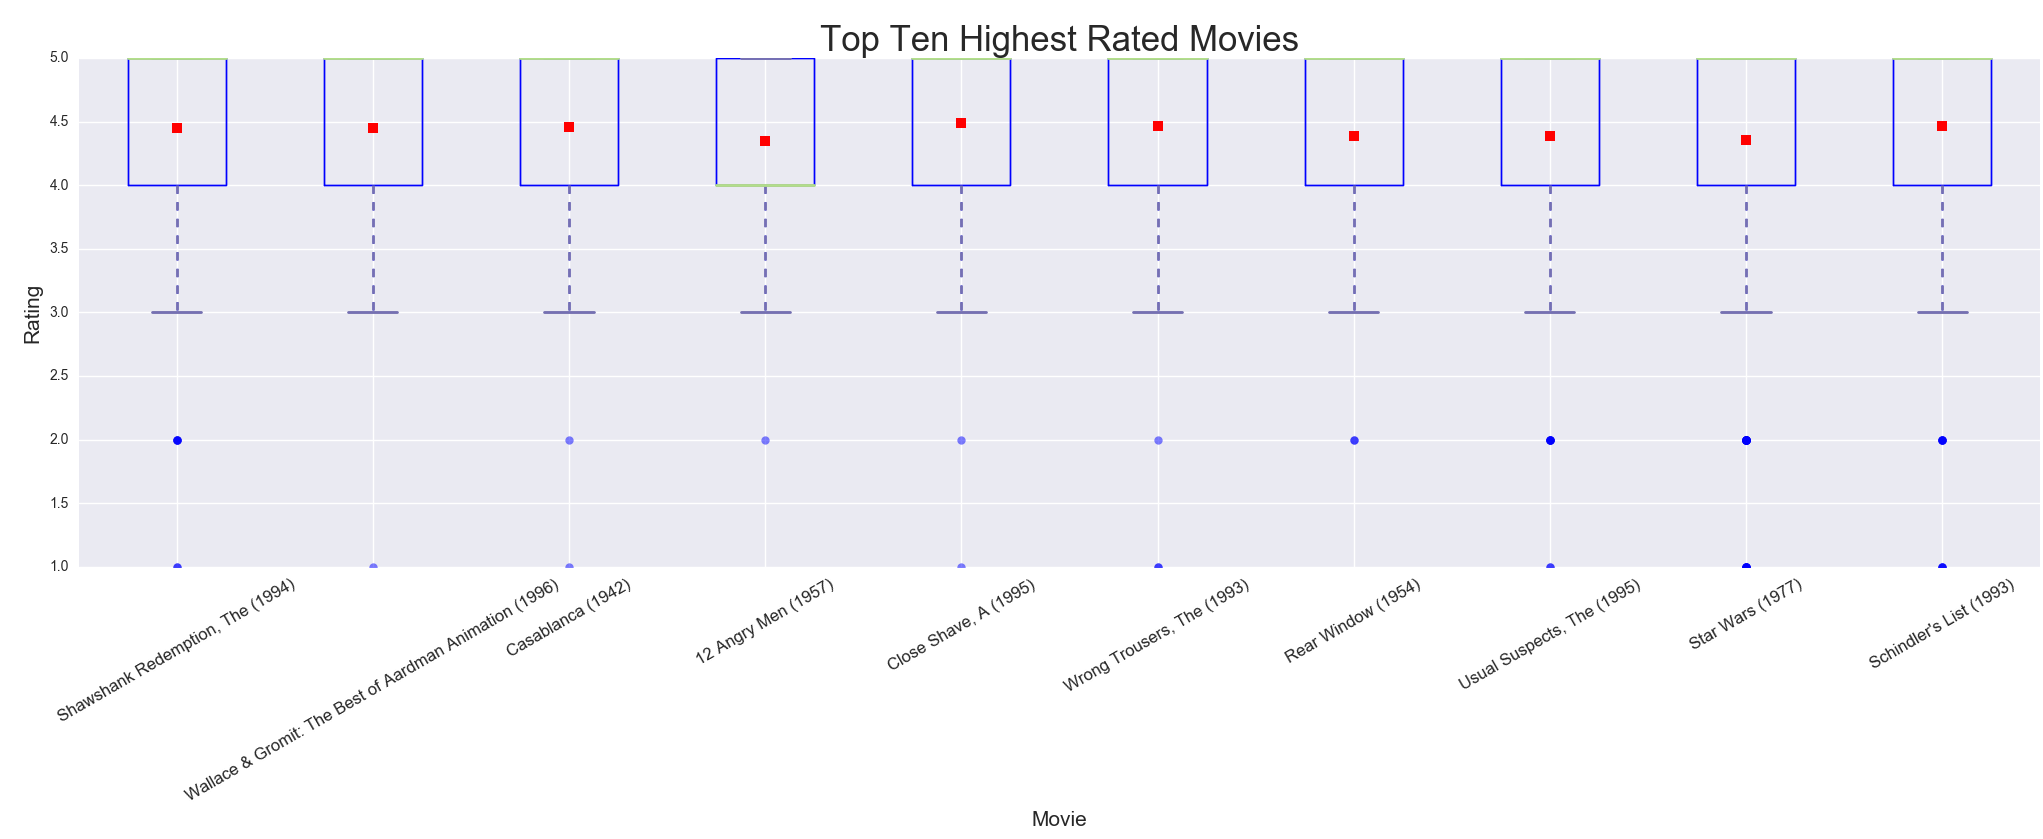
\includegraphics[width=\textwidth]{TopTenHighestRatedBox}
	\caption{Ten most highly rated movies}
\end{figure}

\begin{figure}[H]
	\centering
	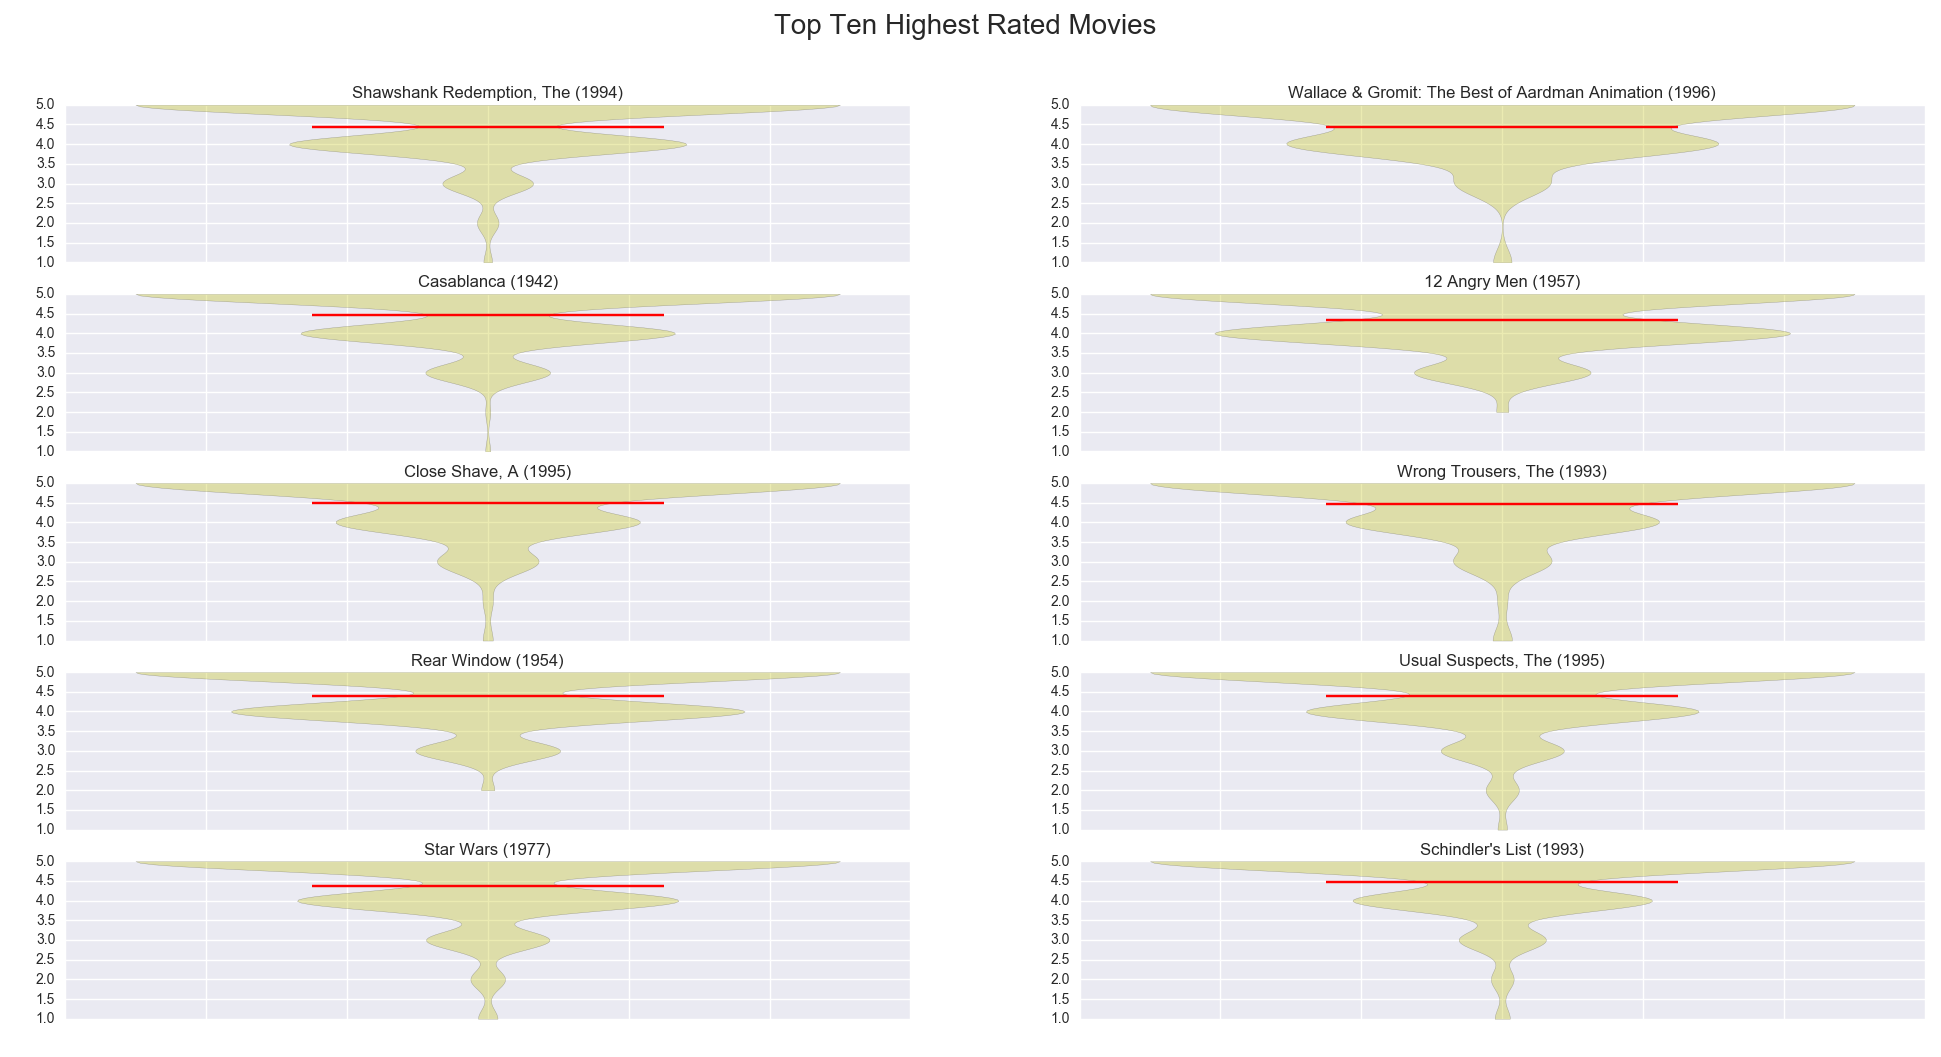
\includegraphics[width=\textwidth]{TopTenBestRatedSwarm}
	\caption{Ten most highly rated movies}
\end{figure}

\noindent It is first important to note that all movies considered in making this list of top ten highest rated movies had more than the median number of ratings per movie in our entire dataset (about 50 ratings). We did not want to consider movies which have less than this number of ratings because there is the possibility of getting a movie which may have an average rating of 5, but have only a handful of ratings. By doing this, we believe we are getting a more accurate representation of what it means for a movie to be ``highly rated."\\

\noindent Similar to the top ten popular movies, we made constructed a box plot and a swarm plot to visualize the distribution of the ten best rated movies. Just comparing the box plots of the most popular(fig. 2) and the best rated (fig. 4), we see a lot less variation in the best rated movies. This is expected, because the popular movies are simply movies with the most ratings, while we obviously expect the highest rated movies to have mainly 5s and 4s. Some, of the movies from the popular list, such as ``Star Wars'' and ``Fargo''��, have distributions very similar to those on the highest rated list, with mean ratings above 4, but the majority of popular movies have distributions that are balanced between high and low ratings. Looking at the swarm plot (fig. 5), we see that the best movies are much higher rated than the most popular movies. Again, the best movies are defined to be as the movies which are rated the highest, so it makes sense that any other distribution of movies will have a lower density of high ratings. 



\subsection*{Genres Comparison: Western vs. Horror vs. Children's Movies}
\begin{figure}[H]
	\centering
	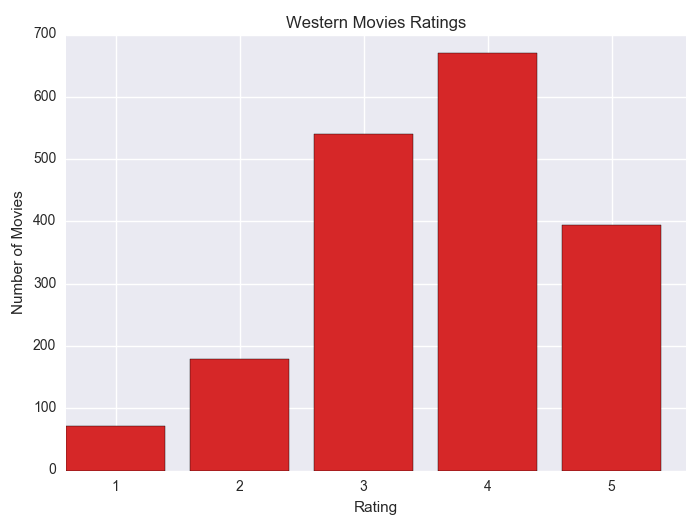
\includegraphics[width=11cm]{BarWestern}
	\caption{Ratings of Western Movies}
\end{figure}

\begin{figure}[H]
	\centering
	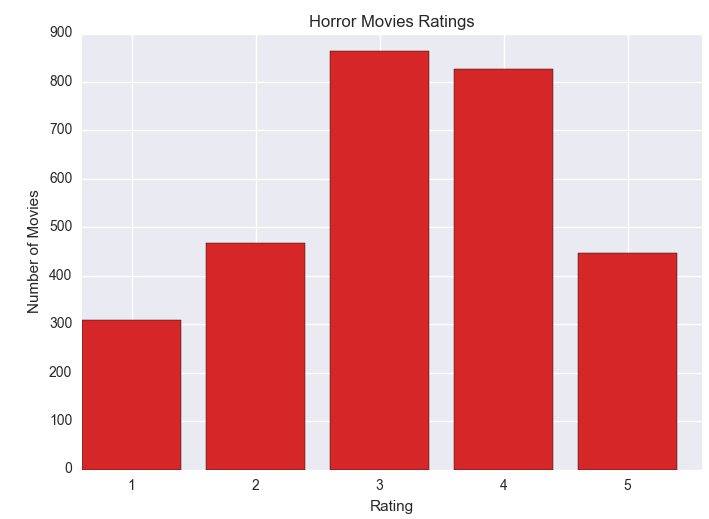
\includegraphics[width=11cm]{BarHorror}
	\caption{Ratings of Horror Movies}
\end{figure}

\begin{figure}[H]
	\centering
	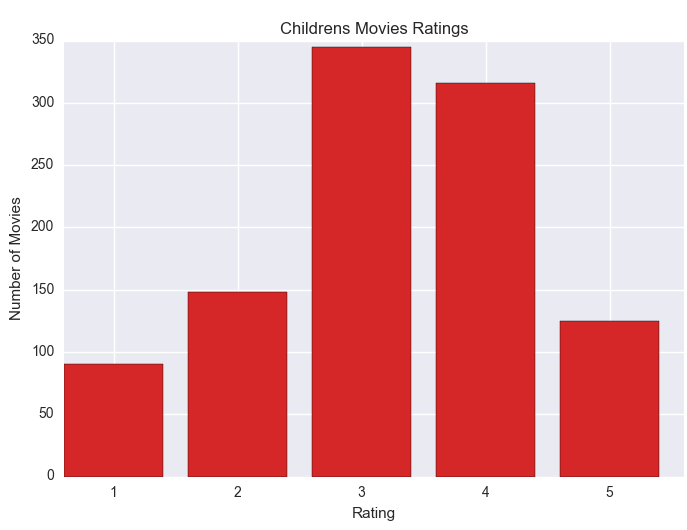
\includegraphics[width=11cm]{BarChildren}
	\caption{Ratings of Children's Movies}
\end{figure}

\noindent To compare ratings between movie genres, we selected children's movies, westerns, and horror movies. In order to directly compare ratings, we first made bar graphs for each genre. In general, we can see that westerns tend to be rated the highest of the three, followed by horror, with children's movies last. Next, to analyze overall distribution of ratings, we constructed box and swarm plots. 

\begin{figure}[H]
	\centering
	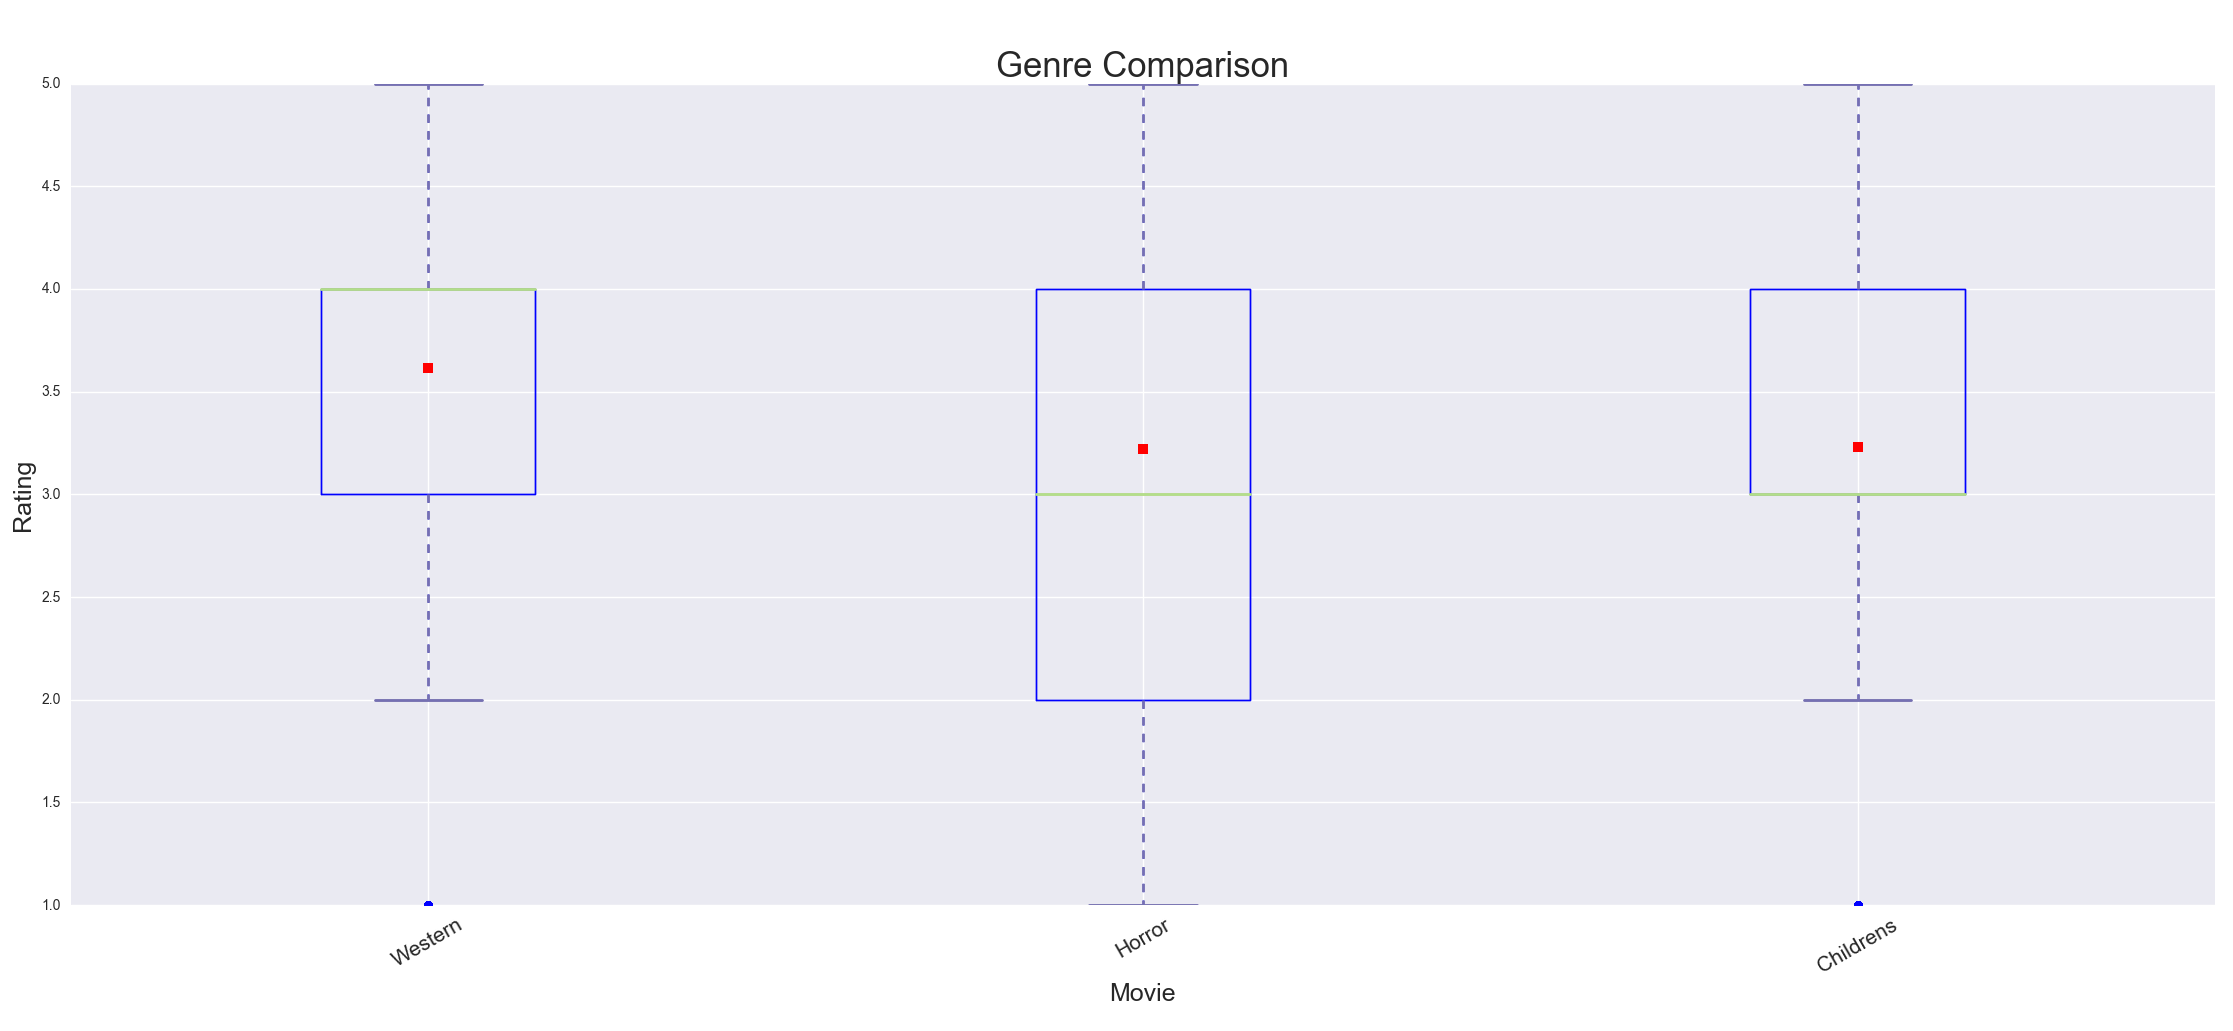
\includegraphics[width=\textwidth]{GenresBoxPlot}
	\caption{Comparing western, horror, and children's movies}
\end{figure}

\begin{figure}[H]
	\centering
	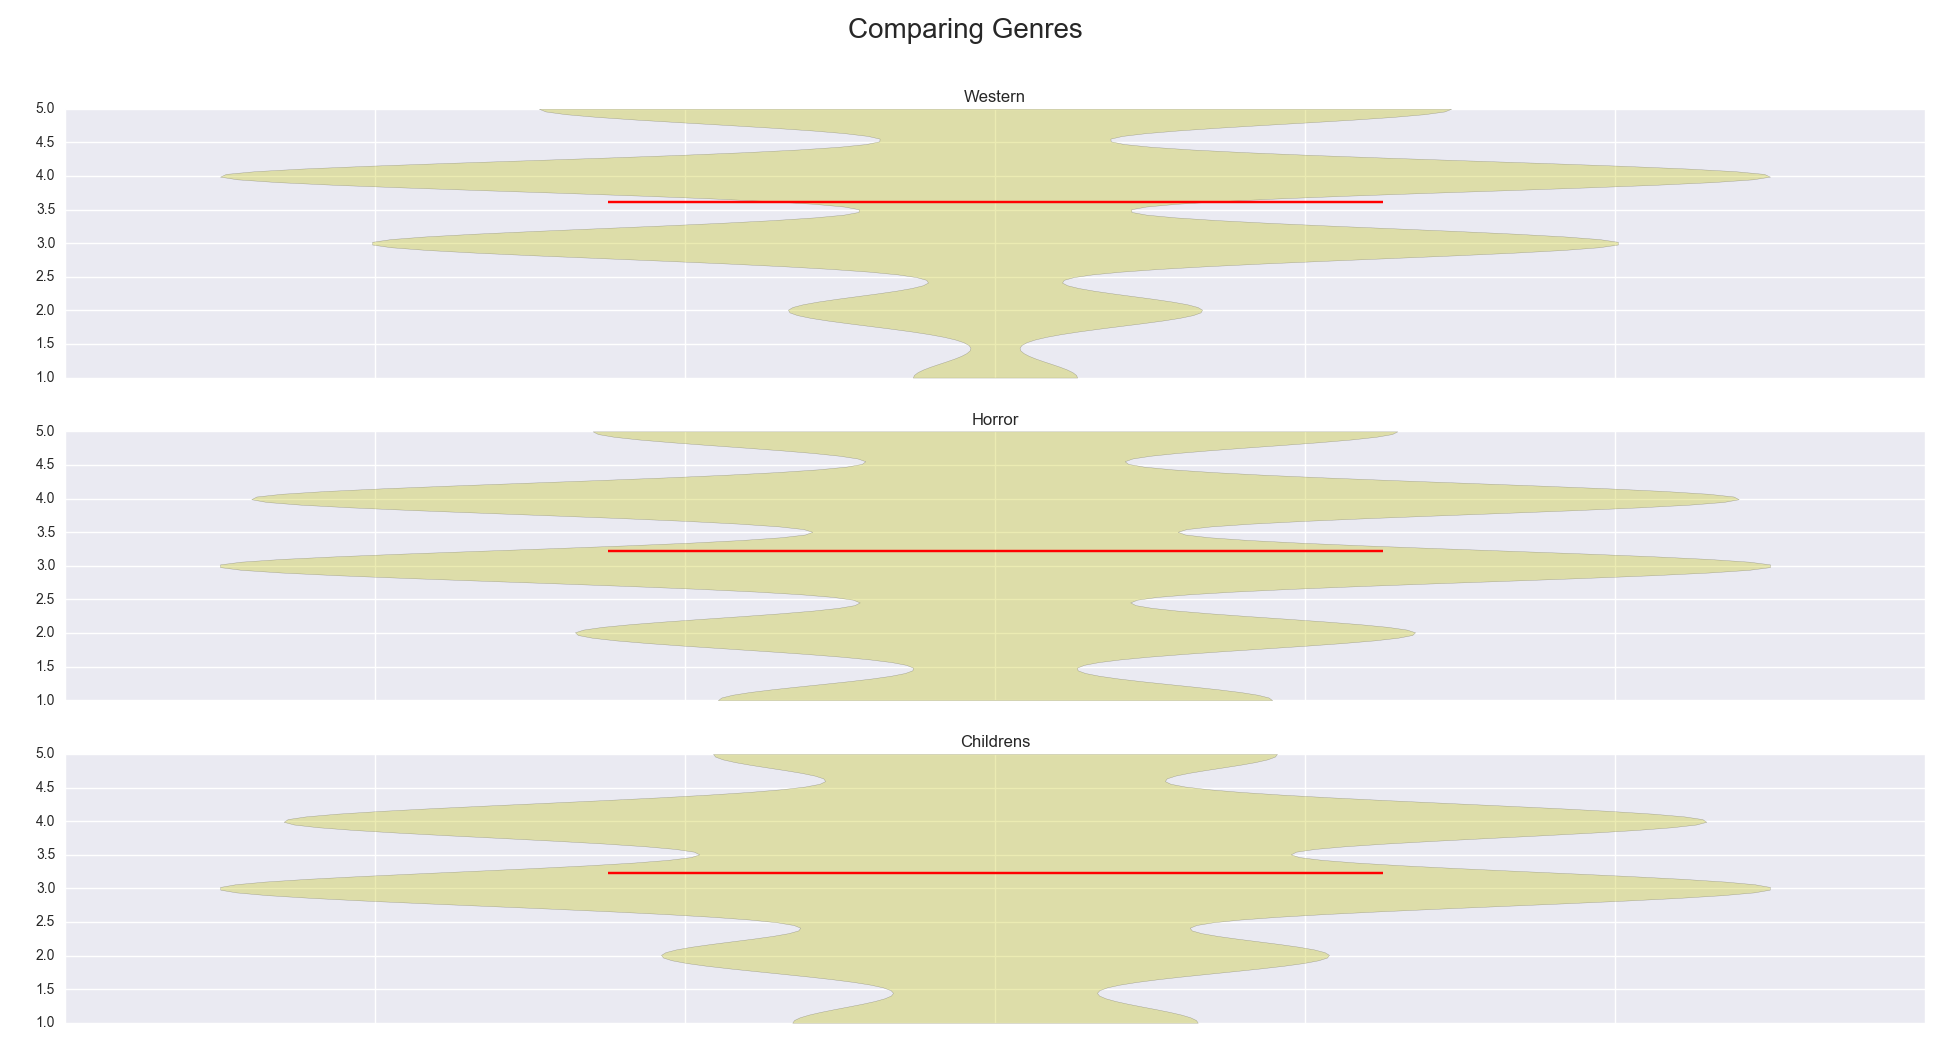
\includegraphics[width=\textwidth]{GenresSwarmPlot}
	\caption{Comparing western, horror, and children's movies}
\end{figure}

\noindent From the box plots (fig. 9) we can see that westerns have a median rating of 4 and a mean of ~3.5, while both horror movies and children's movies have a median of 3 and mean just above 3. From the swarm plots (fig. 10), we can see that westerns are mainly rated 4 with a few 3s and 5s and almost no 2s or 1s. Horror movies tend to have both many good and many bad ratings, while children's movies all tend to have mediocre ratings. This supports our claim that westerns tend to be rated the highest of the three, followed by horror, and then children's.


\section*{Matrix Factorization Visualizations}
From the results of homework 6, we concluded that regularization constant $\lambda = 0.1$ is a good choice for minimizing out-of-sample loss. After some experimentation, we found $\eta = 0.04$ to be the best step size, in that it allowed for the quickest convergence of all step sizes we tested. Our stopping condition was when the difference in training loss from the two most recent epochs was $1/\epsilon = 10^{5}$ times smaller than the difference between initial loss, and loss after the first epoch. Additionally, we capped iterations at 1.5 million, or 15 epochs. We found these stopping conditions effective in letting loss converge to a minimum. Lastly, we used $k = 20$ latent factors, as specified in the assignment. \\

\noindent In general, when viewing visualizations of Matrix Factorizations, we can observe that similar movies tend to be clustered together. This is most evident in our plot of the 10 movies of our choice (fig. 11). We picked 5 science fiction movies, 3 mafia movies and 2 others not in either genre. We observed that the science fiction and mafia movies each had their own cluster, while the 2 others were far away from any other data point. For this plot, we might guess that the x-axis represents seriousness of the film, while the y-axis corresponds to action.

\begin{figure}[H]
	\centering
	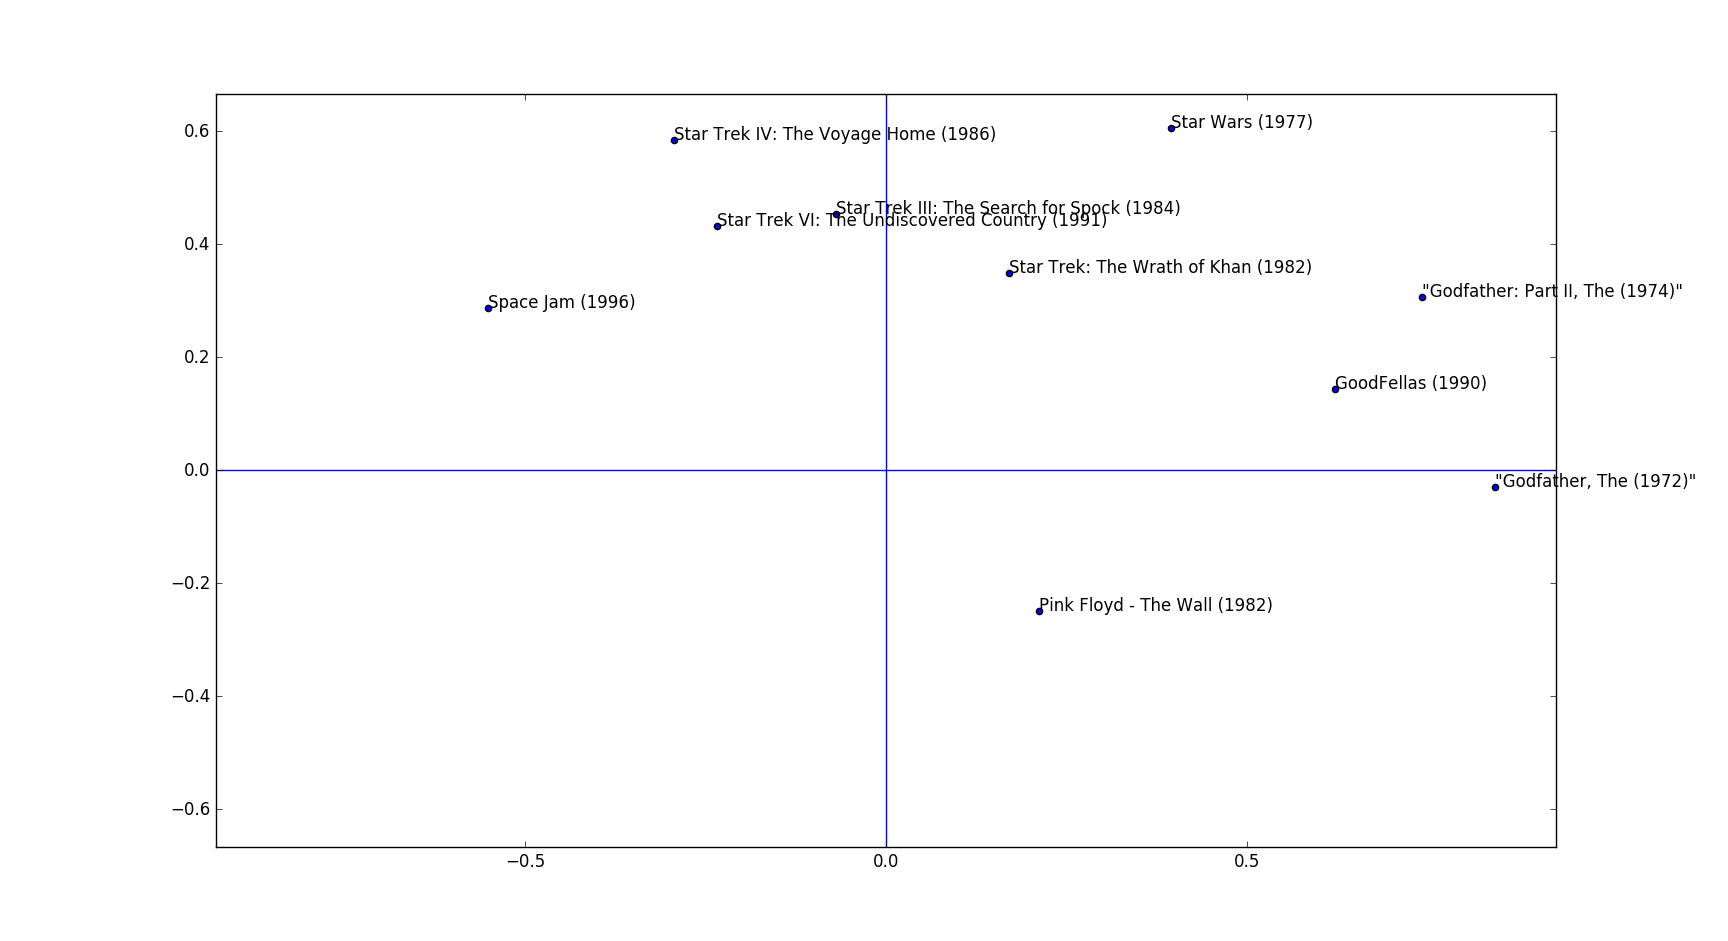
\includegraphics[width=\textwidth]{chosen.png}
	\caption{We choose 5 science fiction, 3 mafia, and 2 movies of other genres.}
\end{figure}

\noindent In the plot of the ten most popular movies (fig. 12), similar movies also tend to be grouped together, as Star Wars and its sequel are near each other, but it is more difficult to interpret the axes. We can also observe that whereas the 10 random movies occupied all 4 quadrants, the most popular movies only occupy the negative y values.

\begin{figure}[H]
	\centering
	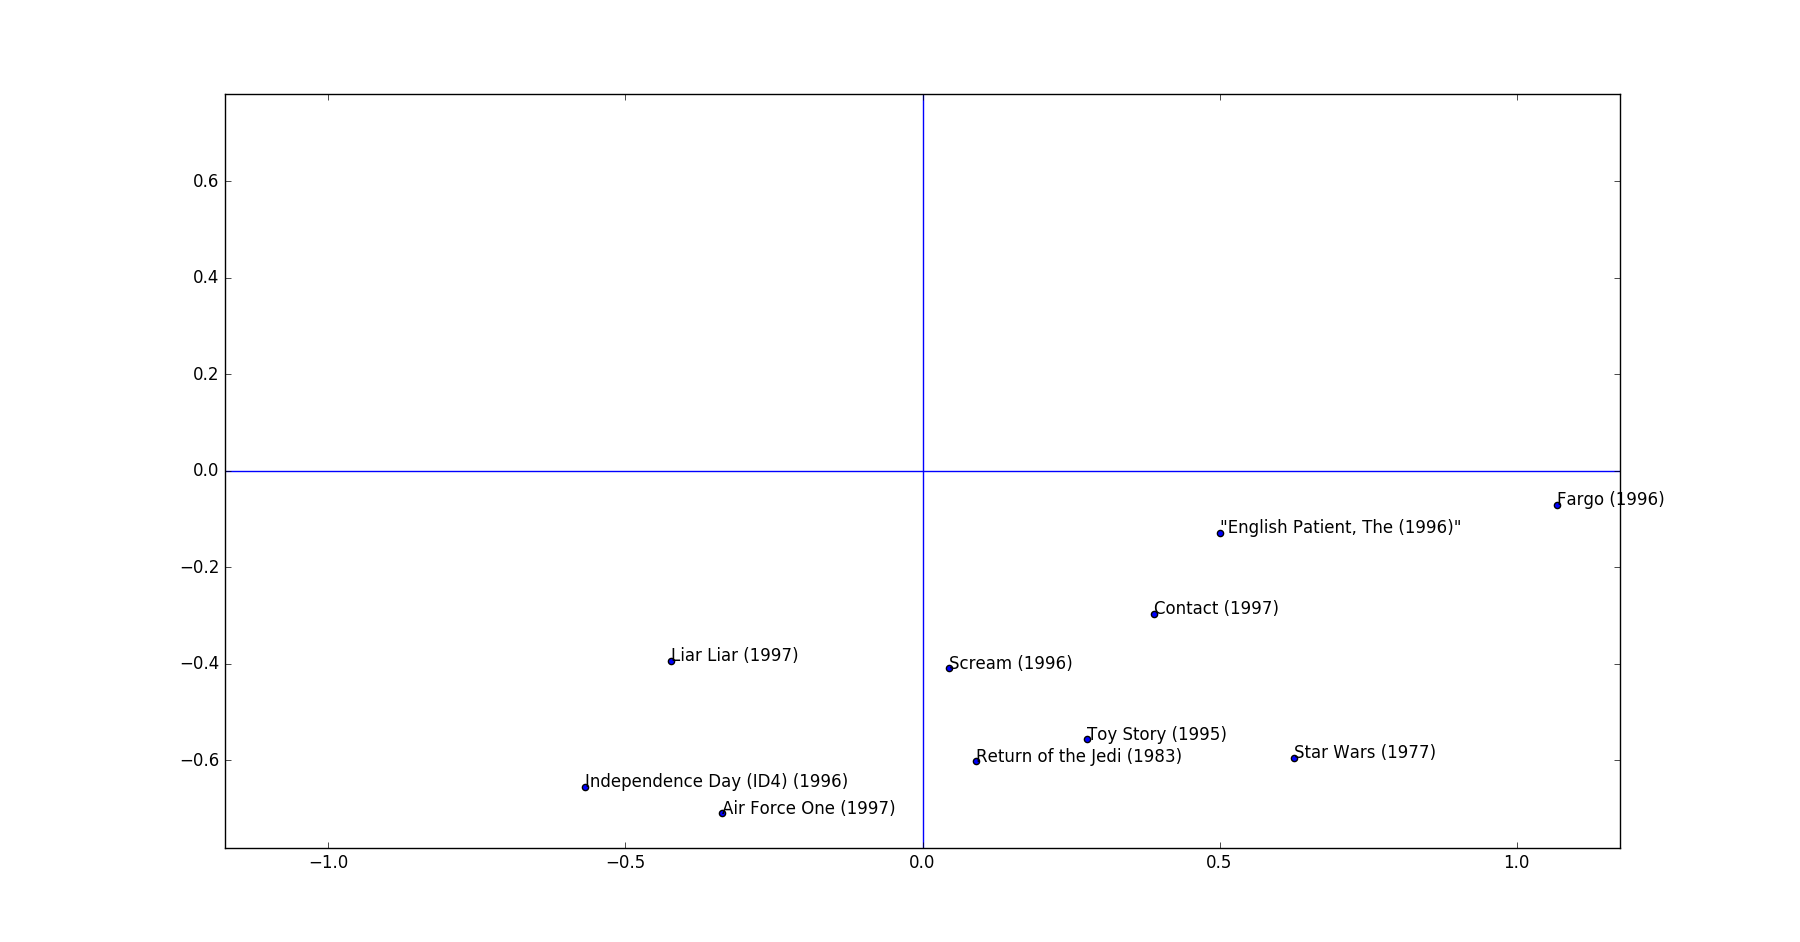
\includegraphics[width=\textwidth]{topTenPopular.png}
	\caption{These are the movies that have accumulated the most ratings.}
\end{figure}
	
\noindent The plot of highest rated movies exhibits the most clustering out of any matrix factorization visualizations. All 10 movies reside in the 4th quadrant very close to each other. This makes some sense because we would expect movies with similar distributions of ratings to be somewhat close. However, this makes interpreting the axes even more difficult than for the plot of the 10 most popular movies.

\begin{figure}[H]
	\centering
	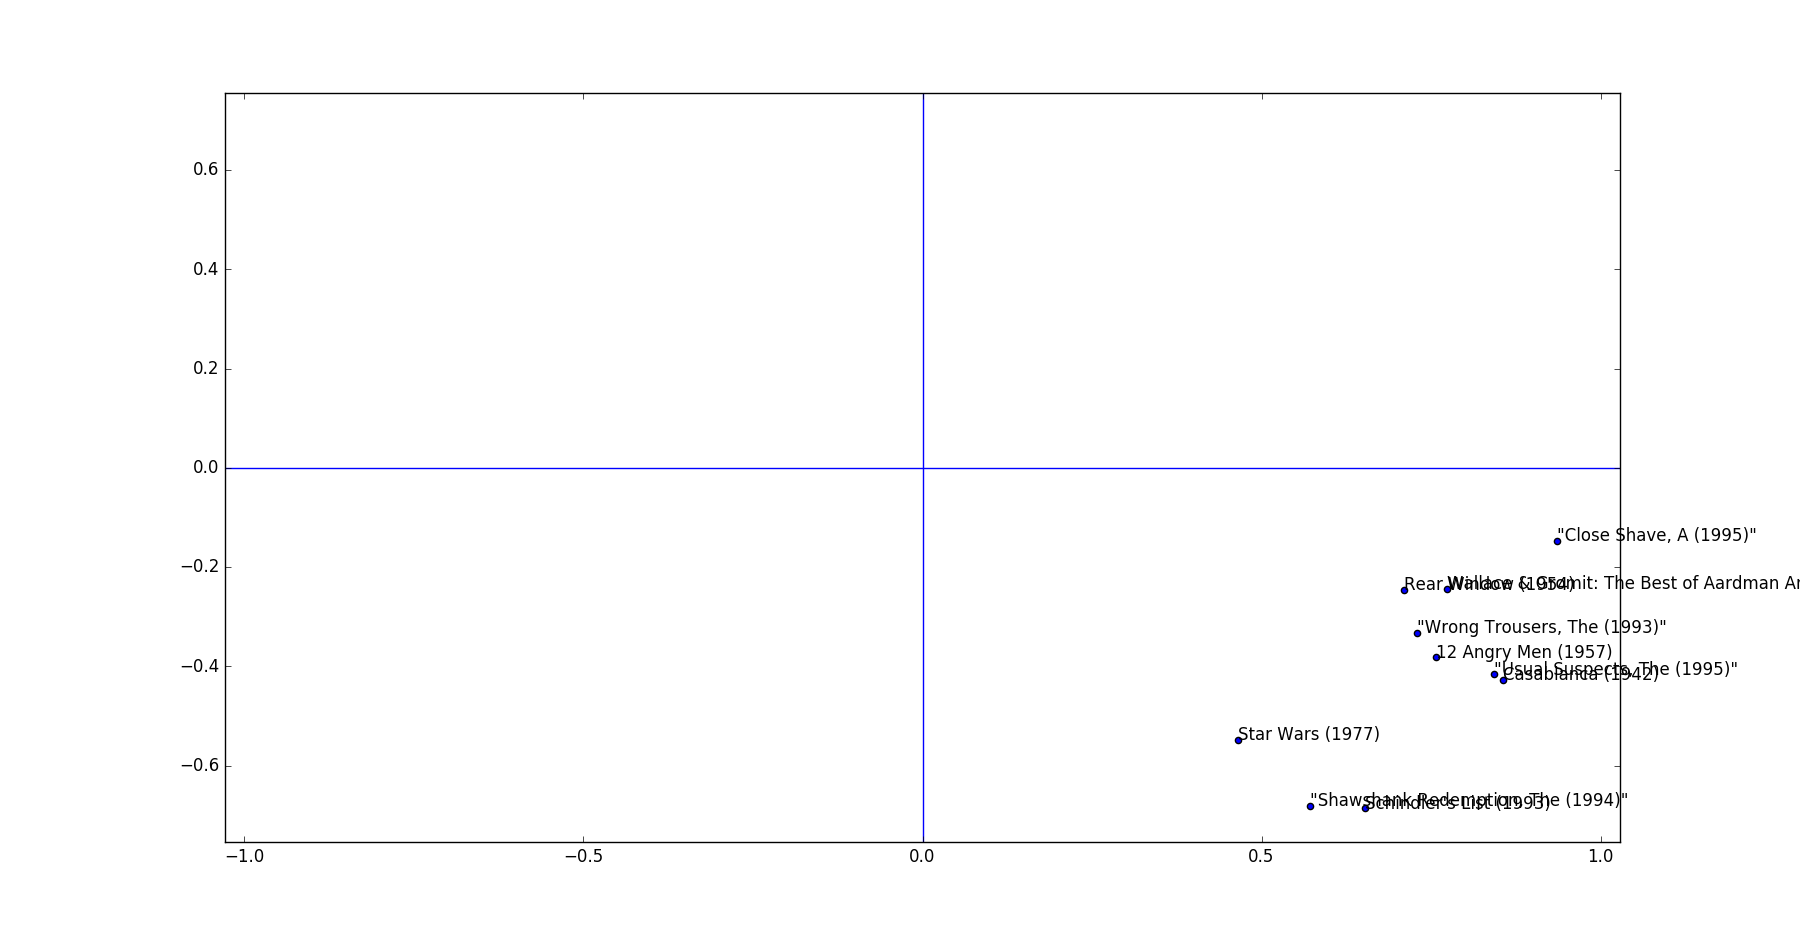
\includegraphics[width=\textwidth]{topTenRated.png}
	\caption{Among movies with at least the median number of ratings, these are the ones with the highest mean rating.}
\end{figure}
	
\noindent When we compare the plots based on the different genres, we see that the data points for Children's movies and Westerns are very clustered together, while the data points for Horror movies are very spread apart. The Children's movies are clustered together except for ``Willy Wonka'' and ``The Wizard of Oz'' which are much less similar thematically than the others. Similarly, for Westerns, most of the movies are alike stylistically, except of ``The Wild Bunch'' and ``Last of the Mohicans,'' and this is represented in the plot. Horror is a very diverse genre, and this is shown by how far apart the points are.

\begin{figure}[H]
	\centering
	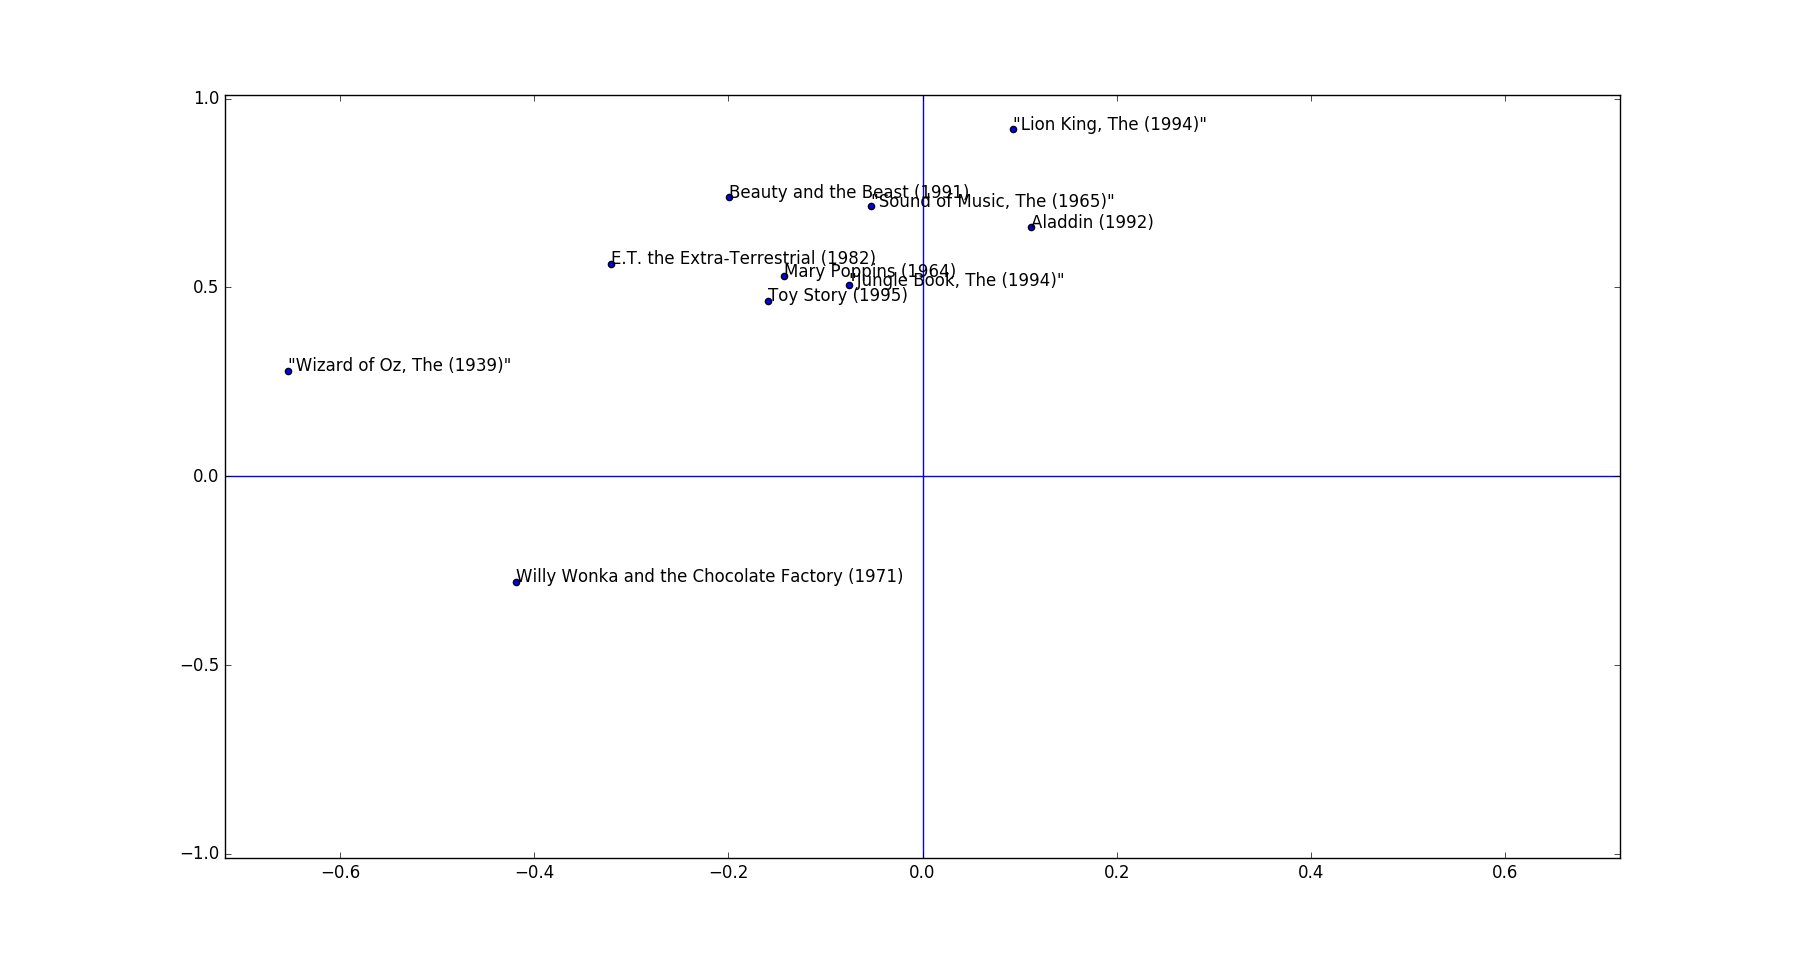
\includegraphics[width=\textwidth]{children.png}
	\caption{This visualization showcases Children's movies.}
\end{figure}

\begin{figure}[H]
	\centering
	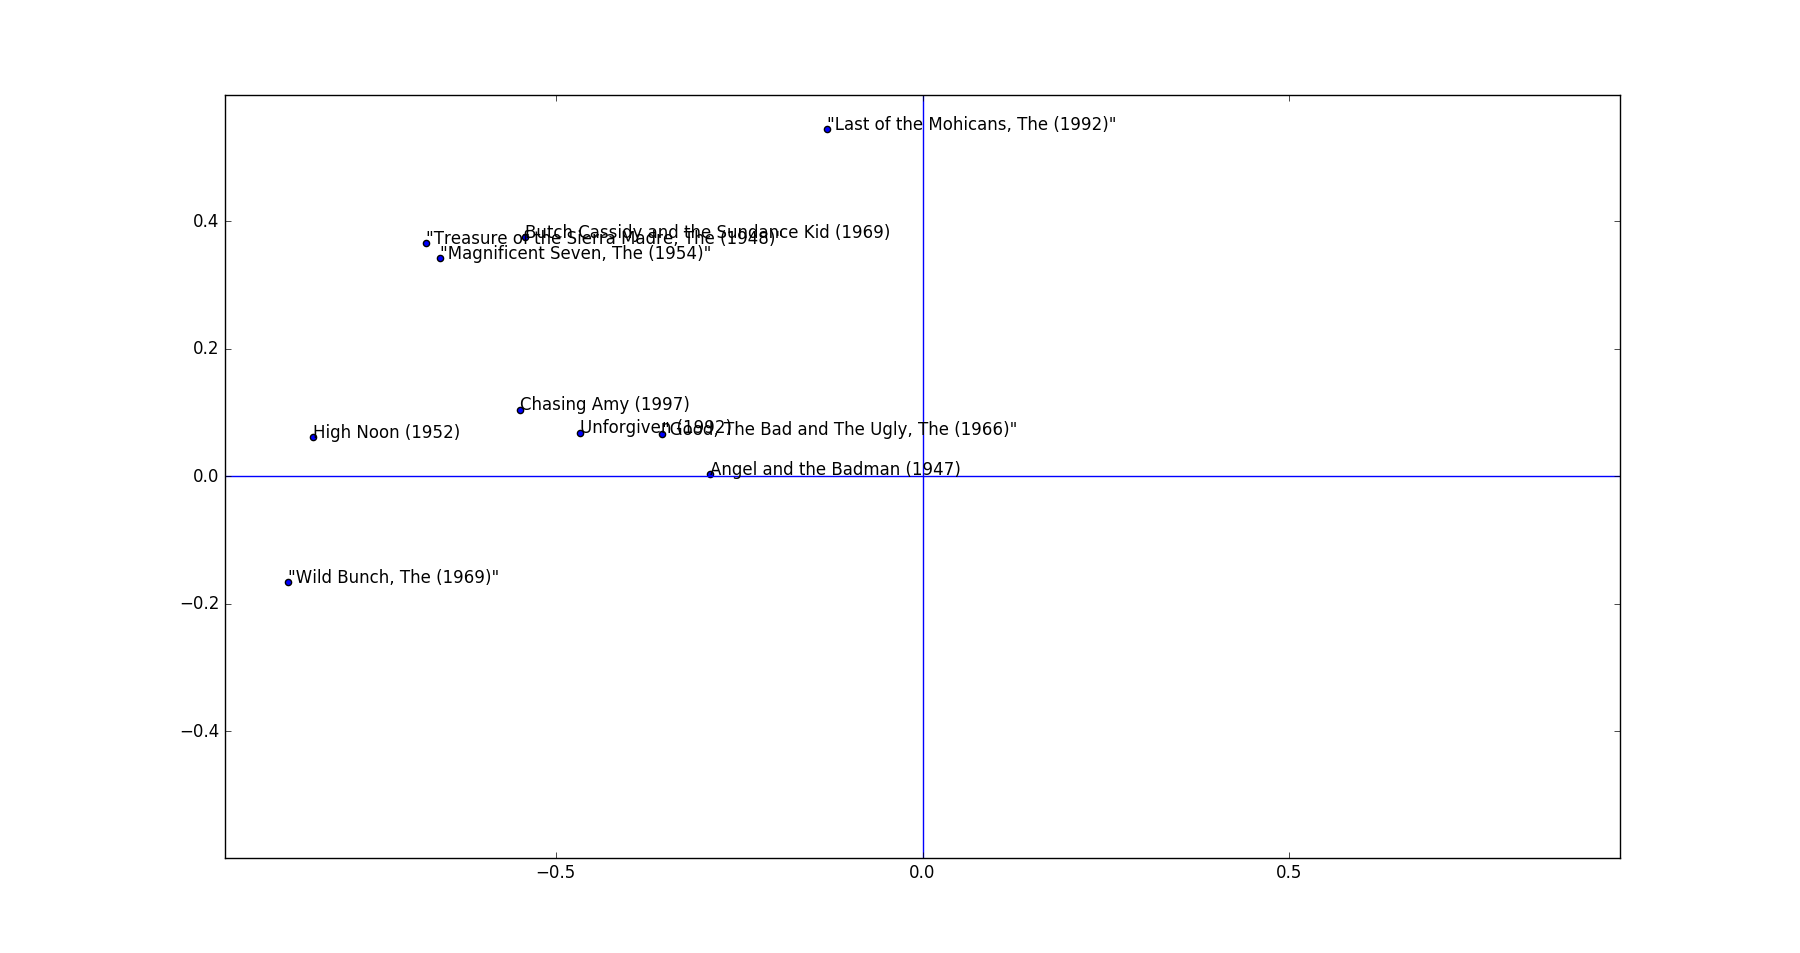
\includegraphics[width=\textwidth]{westerns.png}
	\caption{This is a visualization of some movies of the Western genre.}
\end{figure}

\begin{figure}[H]
	\centering
	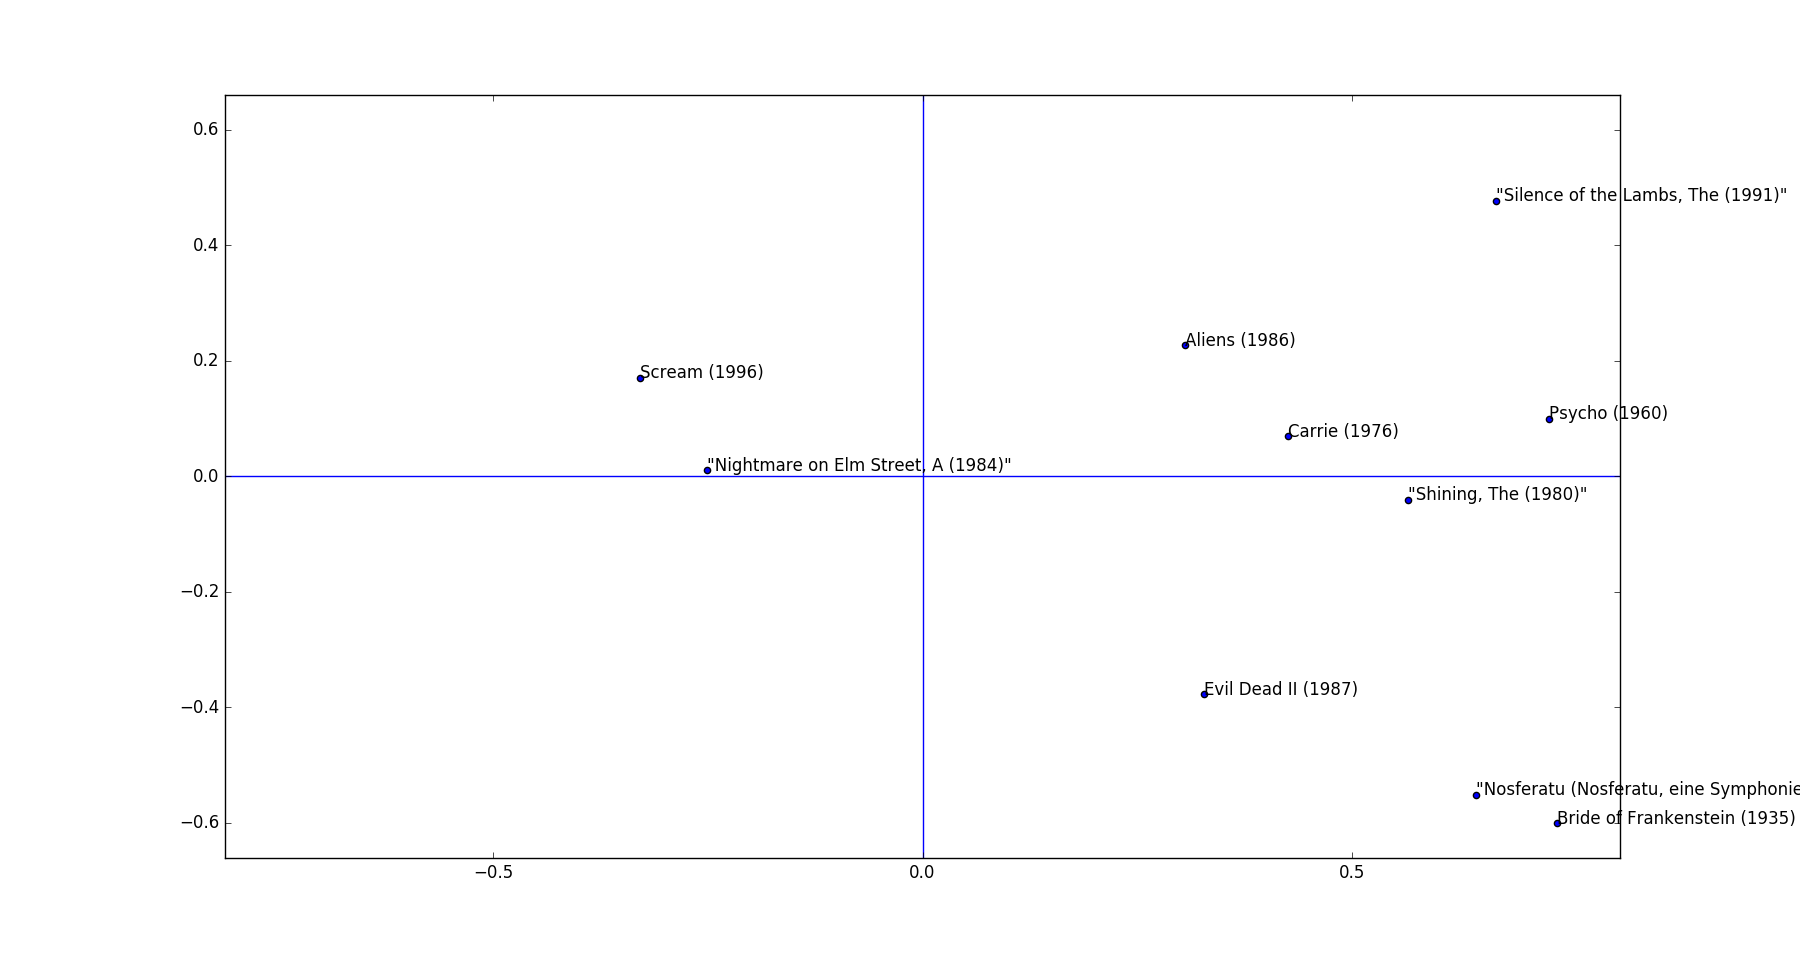
\includegraphics[width=\textwidth]{Horror2.png}
	\caption{These movies are all of the Horror genre.}
\end{figure}

\section*{Conclusion}
For the basic visualizations section, a few of the observations we made were that movies from the top ten most popular were not the highest rated; some had mean ratings hovering around 3.0, and only two had means significantly above 4.0. Additionally, we noticed that the most common rating was 4, followed by 3, and then 5. We agreed that these results are to be expected, because people tend to watch movies they think they will like. We also found that Westerns tend to the highest rated of the three genres, followed by Horror and then Children's. \\

\noindent The general trend that we observed in the matrix factorization visualizations is that similar moves form clusters in this 2-D representation with axes defined by the two ``most important'' characteristics of the dataset, whatever those characteristics may be. While this gave us a much better understanding of this dataset and the idea of PCA and SVD, we were generally unsurprised by the visualizations, in that there were clusters where we expected clusters. However, we at times found difficulty in interpreting the axes, especially for the graph of the most popular movies (fig. 13), in which there were two clusters in the bottom-right quadrant. 
\end{document}